% Preamble
\documentclass[11pt]{article}

% Packages
\usepackage{amsmath}
\usepackage{mathtools}
\usepackage{ragged2e}
\usepackage [utf8]{inputenc}
\usepackage{blindtext}
\usepackage{wrapfig}
\usepackage{xcolor}
\usepackage {polski}
\usepackage{multicol}
\usepackage[a4paper, total={5.7in, 8in}]{geometry}
\usepackage{graphicx}
\usepackage{amstex}
\usepackage{csvsimple}
\usepackage{changepage}
\usepackage{enumitem}
\usepackage[english]{babel}
\usepackage{biblatex}
\usepackage{caption}
\usepackage{indentfirst}
\usepackage{epstopdf-base}
\usepackage{textcomp}
\usepackage{wasysym}

% Document
\begin{document}
%    Nagłówek
    \begin{flushleft}
        Maciej Pierzchała 282 934 \hfill Data wykonania ćwiczenia:\\
        Filip Kubecki 272 655 \hfill 19 listopada 2024r\\
        Grupa: Wtorek 10:35 \\
    \end{flushleft}
    \begin{center}
        \Large\textbf{Laboratorium 6}\\
        \textbf{Charakteryzacja czujników elektrochemicznych}
    \end{center}
    \hfill
%    Treść
    \section{Spis przyrządów}
    \par{
        Do wykonania ćwiczenia wykorzystano:
        \begin{itemize}
            \setlength\itemsep{0em}
            \item[-] Multimetr cyfrowy Sigilent SDM 3055
            \item[-] Termohigrobarometr LAB-EL LB706B
            \item[-] Elektrochemiczny czujnik dwutlenku węgla - TGS4160
            \item[-] Szalki petriego
            \item[-] Pipete automatyczną
            \item[-] Eksykator (objętość $2.75[dm^3]$)
            \item[-] Węglan Sodu - $Na_2CO_3$
            \item[-] Kwas Siarkowy 25\% - $H_{2}SO_4$
        \end{itemize}
    }
    \section{Przebieg i cele doświadczenia}
    \par Ćwiczenie polegało na przygotowaniu odpowiedniej atmosfery badawczej, zawierającej odpowiednią koncentrację
    dwutlenku węgla $CO_{2}$. Następnie należało zmierzyć zawartość $CO_2$ w każdej atmosferze przy pomocy czujnika elektrochemicznego.\\
    \indent Na podstawie pomiarów należało wyznaczyć stężenie dla nieopisanej atmosfery badawczej oraz wyznaczyć przewidywane stężenie tej atmosfery
    na podstawie ilości wykorzystanego Węglanu Sodu oraz wzoru stechiometrycznego reakcji. Należało również wyliczyć liczbę moli oraz ciśnienie cząstkowe
    $CO_2$ atmosfery badawczej.

    \section{Obliczenia i analiza wyników}
    \par Na podstawie stężenia molowego Węglanu Sodu oraz jego objętości wykorzystanej dla każdej atmosfery badawczej wyznaczono ilość moli Węglanu Sodu
    wykorzystanych w reakcji:
    \begin{gather}
        C_{NA_{2}CO_{3}}=\frac{n_{NA_{2}CO_{3}}}{V}=\frac{1[mol]}{1000[ml]}
    \end{gather}
    \noindent Przykładowo dla atmosfery nieznanej dal której wykorzystano $0.4[ml]$ Węglanu Sodu wykorzystując proporcję obliczamy że:
    \begin{gather}
        \frac{1[mol]}{1000[ml]}=\frac{X}{0.4[ml]} \\
        X=\frac{1[mol]\cdot 0.4[ml]}{1000[ml]}=0.0004[mol]
    \end{gather}
    \noindent Na podstawie równania stechiometrycznego reakcji umieszczonego poniżej możemy zauważyć że ilość substratów reakcji zmienia się liniowo
    wraz ze zmianą produktów. Jednocześnie ilość moli produktów (oddzielnie Węglanu Sodu i Kwasu Siarkowego - nie ich sumy) jest równa ilości moli
    substratów więc ilość moli Węglanu Sodu będzie równa ilość moli wyprodukowanego dwutlenku węgla.
    \begin{gather}
        NA_{2}CO_{3}+H_{2}SO_{4}\rightarrow CO_{2}\uparrow+NA_{2}SO_{4}+H_{2}O
    \end{gather}
    \noindent Na na podstawie równania Clapeyrona jesteśmy w stanie obliczyć objętość wyprodukowanego $CO_2$:
    \begin{gather}
        pV=nRT \\
        V=\frac{nRT}{p}
    \end{gather}
    \noindent Podstawiając wyliczoną ilość moli $CO_2$, stałe oraz parametry sali badawczej, wyliczamy objętość gazu (przykład dla atmosfery nieznanej):
    \begin{gather}
        V_{CO_2}=\frac{0.0004[mol]\cdot 8.314[mol\cdot K]\cdot 296.6[K]}{98320[Pa]}=1.003227177\cdot 10^{-5}[m^3]
    \end{gather}
    \noindent Znając objętość powstałego $CO_2$ oraz objętość eksykatora ($2.75[dm^3]$), możemy wyliczyć stężenie $CO_2$:
    \begin{gather}
        x_{CO_2}=\frac{V_{CO_2}}{V_{ekskatora}}\cdot 10^6[ppm]
    \end{gather}
    \noindent Dla nieznanej atmosfery:
    \begin{gather}
        x_{CO_2}=\frac{1.003227177[m^3]}{2.75[dm^3]}\cdot 10^6[ppm]=\frac{1.003227177[m^3]}{0.00275[m^3]}\cdot 10^6[ppm]=3648.099[ppm]
    \end{gather}
    \noindent Przy pomocy poniższego równania obliczamy ciśnienie cząstkowe dwutlenku węgla:
    \begin{gather}
        p_{CO_2}=\frac{X_{CO_2}}{10^6}\cdot p_{atm}
    \end{gather}
    \noindent Dla nieznanej atmosfery:
    \begin{gather}
        p_{CO_2}=\frac{3648.099[ppm]}{10^6}\cdot 98320[Pa]=358.6811[Pa]
    \end{gather}
    \noindent Poniżej zamieszczono tabelę zawierającą wyniki powyższych pomiarów dla wszystkich atmosfer:
    \subsection{Tabela 1}
    \begin{center}
        \Large\csvreader[tabular = |c|c|c|c|,
            table head = \hline  \boldmath{$x_{CO_2}[ppm]$}  & \boldmath{$N_{CO_2}[mol]$} & \boldmath{$x_{cCO_2}[ppm]$}  & \boldmath{$P_{CO_2}[Pa]$}  \\\hline,
            late after line = \\\hline
        ]{Data/output.csv}{}{
            \csvcolii & \csvcoliii & \csvcoliv & \csvcolv
        }
    \end{center}
    \indent Na podstawie pozyższych danych wykreślono zależność $SEM=f(log(P_{CO_2}))$:\\


    \noindent\makebox[\textwidth]{
        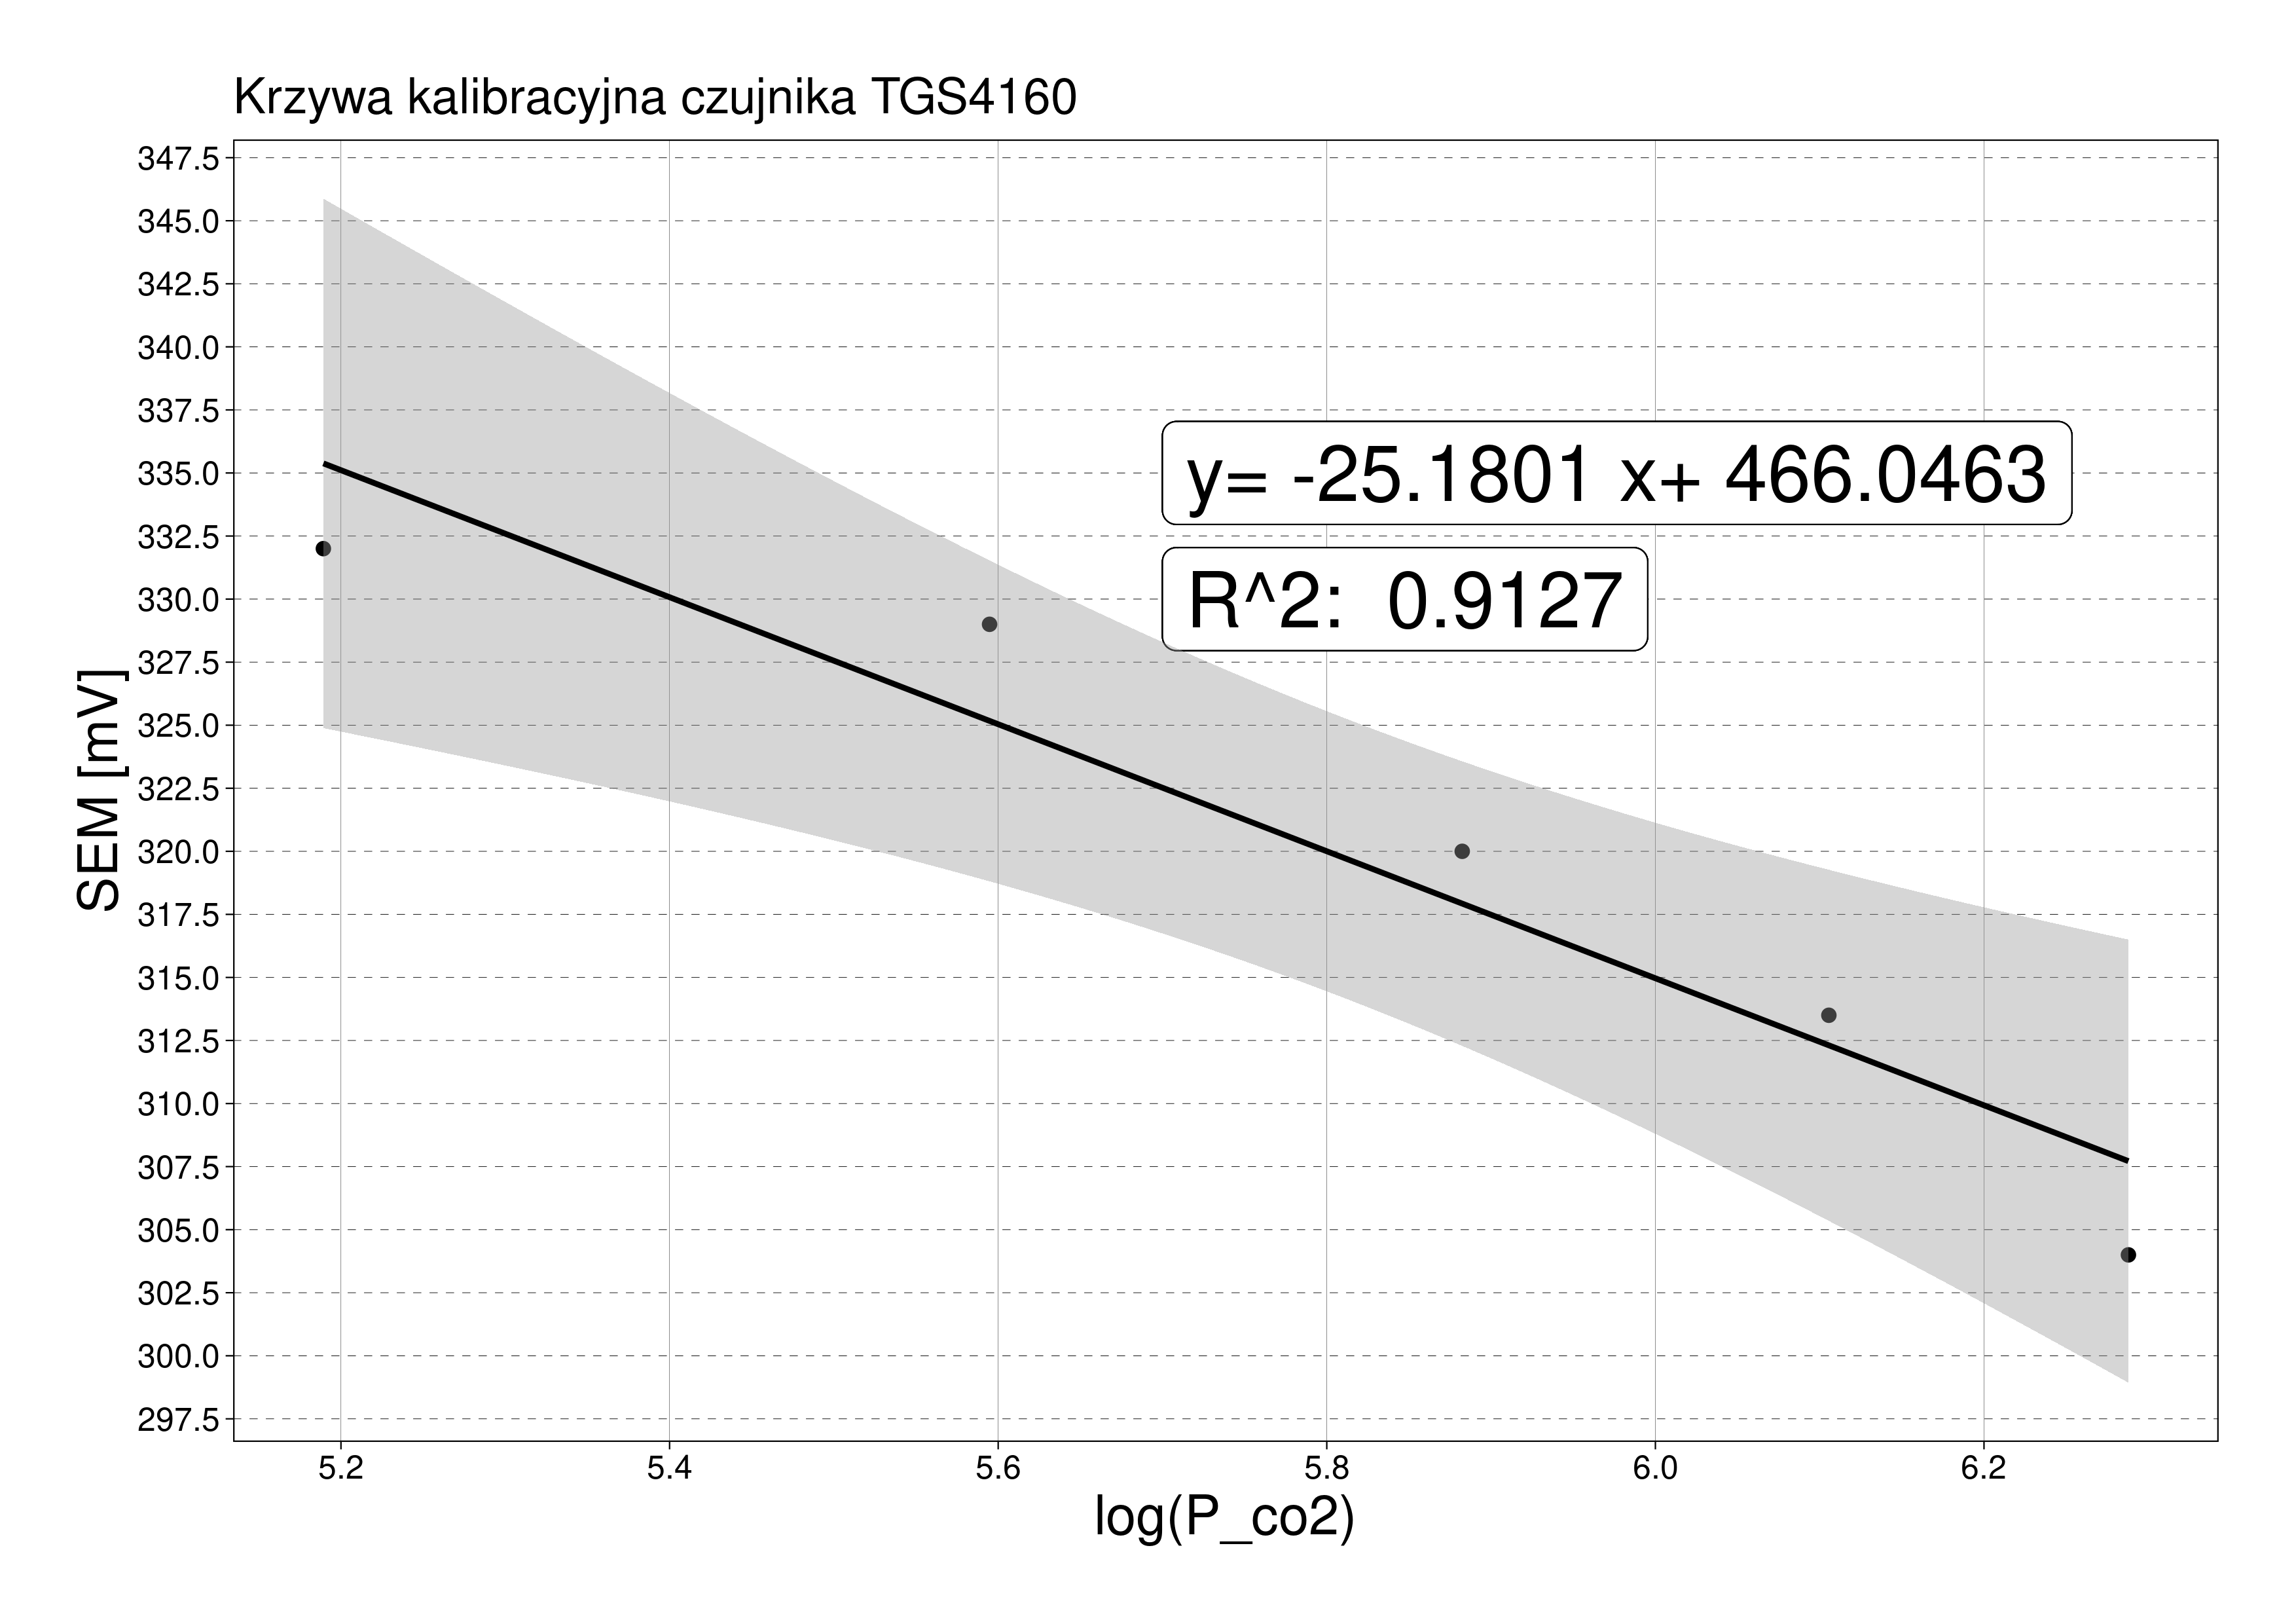
\includegraphics[scale = 0.7]{/home/bork/IdeaProjects/LatexProjects/src/PodstawyTechnikiSensorowej/Lab6/Img/plot1}}
%    \begin{gather*}
%        T_{rise}=52.54[s]\\
%        T_{fall}=3.99[s]
%    \end{gather*}
%    \subsection{Tabela 1}
%    \begin{center}
%        \Large\csvreader[tabular = |c|c|c|c|c|,
%            table head = \hline  \textbf{$x_{gaz}[ppm]$}  & \textbf{$R[k\Omega]$} & \textbf{$I_{max}[\mu A]$}  & \textbf{$G[S]$} & \textbf{$S$}  \\\hline,
%            late after line = \\\hline
%        ]{Data/output.csv}{}{
%            \csvcolii & \csvcoliii & \csvcoliv & \csvcolv  & \csvcolvi
%        }
%    \end{center}
    \section{Wnioski}
    \par Z powodu braku danych z programu mierzącego bezpośrednio $SEM$ czujnika nie udało się wykreślić wykres $SEM=f(t)$ oraz wyznaczyć
    czas odpowiedzi oraz czas powrotu. Niemiałoby to jednak większego znaczenia gdyż dla pomiarów wykonywanych w naszym zestawieniu badawczym
    odczyty czujnika zaczynały spadać już po kilku sekundach pomiaru. Mogło to być spowodowane nieszczelnym eksykatorem (wymuszony stan z powodu przewodu
    znajdującego się pod nakryciem naczynia). Mimo posiadania tego typu danych wyniki byłby nieprawidłowe gdyż nota katalogowa mówi o $2[min]$ czasie
    odczytu czujnika.\\
    \indent Obliczenia ciśnienia parcjalnego i ilości cząsteczek $CO_2$ są zbliżone do wartości podanych w tabeli. Odbiegają one maksymalnie o $200[ppm]$
    dla największych wartości co wynikać może z różnych parametrów otoczenia dla których wartości te zostały obliczone.\\
    \indent Charakterystyka czujnika mimo przelogarytmowania wartości $x_{CO_2}$ dalej nie jest idealnie liniowa. Współczynnik $R^2$ dla regresji
    liniowej wynosił jedynie $91.27\%$. Nie jesteśmy pewni powodów tego problemu. Możliwe jest iż układ pomiarowy lub czujniki wymagają zmiany.\\
    \indent Kluczowym jest to iż udało się wyznaczyć ilość cząsteczek $CO_2$ dla nieznanej atmosfery. Wartość ta wynosi $3648.1[ppm]$ co patrząc na
    pozostałe pomiary oraz charakterystykę czujnika powinno być bliskie prawdy.


%    %Bibliografia
%    \vfill
%    \footnotesize
%    \begin{thebibliography}{3}
%        \bibitem{texbook1}
%        https://en.wikipedia.org/wiki/Reactivity-selectivity\_principle
%        \bibitem{texbook2}
%        https://en.wikipedia.org/wiki/Breathalyzer
%        \bibitem{texbook3}
%        https://www.olythe.io/alcohol-unit-converter
%        \bibitem{texbook4}
%        https://en.wikipedia.org/wiki/Fuel\_cell
%    \end{thebibliography}
\end{document}
